\chapter{无监督的自举式情感分类}
\label{ch4}

\section{引言}
\label{ch4_intr}
文本的情感分析是挖掘文本中主观性信息学的主要手段,是研究文本中观点、态度、情绪和立场等主观性信息是如何表达的。情感分析技术可以从数量庞大的文本数据中抽取并总结主观性信息,为后续的一些应用(商业智能(Business Intelligence),舆情分析(Public Opinion Analysis)或选举预测(Election Prediction)等)提供技术和工具支持\upcite{Liu2012}。在社交媒体中,一些基于文本的平台比如微博产生了大量针对各种话题或实体的带有主观性信息的数据。这对这些数据的分析,也就是情感分析正逐渐受到各个研究领域(比如推荐系统和搜索引擎)的重视。情感分析中一个主要的方法就是应用各种分类技术,也就是根据作者的主观态度将文本进行分类,一般将这种研究称为情感分类研究。情感分类一般是从一些标注过的训练数据中通过学习得到一个分类模型,学习得到能够将一种情感类型区别于其他类型的一些特征\upcite{LourencoJr2014}。这种模型的性能主要依赖于其能够学习到的数据中出现的情感的文本表达模式,一般是文本中出现的词语、短语或者词语的各种组合。情感分类也就是情感分析的分类形式,虽然可以被视作文本分类的特殊形式,实际上情感分类是比文本分类更具挑战的任务,因为文本中情感的表达方式严重依赖领域和上下文环境\upcite{Jiang2011}。

随着微博(Twitter、新浪微博等)的出现和广泛使用,用户产生内容(UGC,User-Generated Content)成指数增长,这些内容并且这些内容对于我们来说是很容易获取的,并且这些内容里面有很多用户对于各种话题的观点和情感等主观性信息。因此我们可以很方便的从这些数据中提取出主观性信息,并使其在商业、旅游或者健康领域得到应用。但是对微博进行情感分类特别具有挑战性,因为(1)用户使用微博表达观点的方式是多种多样的,既有正规传统语言的表达方式,又有社交媒体特有的流行的表达方式,比如“coooooool、OMG、:-(、屌丝、逆袭”等,这些表达方式虽然对于人来说是比较直观和易于理解的,并且更加方便了用户的在线交流,但是对于计算机来说,却是很难准确确定这些表达方式的观点和情感等语义信息。(2)更具挑战性的是,因为用户群体的复杂性,经常会有用户创造出的一些缩写词或者新词,并且会将一些传统的词赋予新的语义在微博中重新使用,这些语言上的变化使得微博上观点的表达方式有别于传统文本的表达方式。综上所述,可以看出微博中的文本噪声、非正式本质以及语言词汇的急剧膨胀使得对微博中表达的主观性信息自动分析需要依赖于微博这种独特的语言环境,因此进行情感分类是困难的。这种情况被称为微博情感分类的领域(或语言环境)依赖问题,也就是使用其他文本数据集(比如评论或博客)训练出的分类器在微博的情感分类时会出现性能急剧下降,而要获得大量微博训练数据集需要大量的人力,并且微博数据具有时效性,不同时间阶段的微博数据集中观点表达方式也会产生漂移。

本章我们主要关注微博情感分类的领域依赖性问题。为了解决这个问题,基于我们的一些观察,我们提出了一种无监督的自举式(bootstrapping)情感分类框架。该框架首先使用现有的已经有情感标签的语言资源训练得到一个通用的能够跨领域使用的分类器;然后再根据该分类器的跨领域特点使用其作为初始分类器对微博进行分类,获得一些高可信度的微博作为训练集训练得到一个微博分类器;将两个分类器结合迭代使用共同训练(Co-training)过程,逐步在目标数据集扩展并训练微博分类器,直至其分类性能达到最优。

\section{相关工作}
\label{ch4_relt}
情感分类在观点挖掘研究中越来越受到重视,前期工作主要研究针对评论(商品或电影)进行情感分类。经常使用的方法可以分为基于规则的方法和基于学习的方法,其中基于机器学习方法性能一般比较好因而常被用来作为对表的标准\upcite{Pang2002}。

现在研究人员逐渐开始注意到微博中用户的主观性信息,并开始结合微博的语言特点进行对微博进行情感分类研究。一些研究显示可以将微博的一些独特的特征结合进情感分类方法中。比如,Barbosa和Feng~\upcite{Barbosa2010}提出了两阶段支持向量机分类器(Support Vector Machine (SVM) classifier)对tweet进行情感分类,证明了该分类其能对tweet的类别偏置(biased)和噪声具有很好的鲁棒性;Hu等~\upcite{Hu2013}将社交媒体数据中的情感表达解成情感指征(emotion indication)和情感关联(emotion correlation)两种信号,通过对两类情感信息进行联合建模方式实现了对微博的无监督情感分类;Jiang等~\upcite{Jiang2011}主要关注依赖于特定目标的微博情感分类,提出了通过将目标依赖特征(target-dependent features)和相关微博同时进行考虑的监督学习方法,并证明了可以提升情感分类性能;Wang等~\upcite{wang2011topic}针对hashtag级别的情感分类进行了研究,并提出了一个全新的图模型,然后使用提升(boosting)式分类方法进一步提高了模型的性能;Amir等~\upcite{AsiaeeT2012}针对单条微博的情感分类提出了一个分层分类器框架,框架通过抽取对特定目标的微博,将微博按情感类型分开以及分离正负情感类型微博三个层次进行有监督的分类学习;Hu等~\upcite{hu2013exploiting}基于社交理论抽取微博之间的情感关系,提出了一种全新的社会学方法使用这些情感关系以促进情感分类性能,并有效解决了数据中的噪声问题;同样受到社会学理论的启发,Guerra等~\upcite{CalaisGuerra2011}依据人类通常会持有一致的带有偏执的观点,提出了全新的迁移学习(transfer learning)方法解决微博基于话题的实时情感分类问题;Thelwall等~\upcite{Thelwall2010,Thelwall2012}设计了SentiStrength情感分析工具,用于对微博等社交媒体中非正式语言中的情感分析,该工具是基于规则的方法,使用了人工编辑的词典并结合了微博语言中的句法和拼写特点抽取微博中的情感强度,该工具获得了广泛的应用。

以上这些工作通过利用微博的一些网络和语言特点对情感分类方法进行了适应性的改进,以使得这些方法能够适用于微博语言环境,但是没有彻底解决微博情感分类问题的语言环境依赖问题,本章我们提出的方法从一个全新的视角来看情感分类问题,将情感分类的特征空间分各位环境依赖部分(context-dependent part)和环境独立部分(context-independent part)分别进行训练分类器,然后将两种分类器结合进一个自举式(bootstrapping)学习框架中。

\section{问题的形式化}
\label{ch4_form}
简单来说,情感分类主要目标就是将文本分类为预先定义的情感极性类别(一般是积极的,positive或消极的,negative)。形式化上,对于给定的文档语料库$ D=\lbrace d_{1},\dots ,d_{n} \rbrace$,预定义的情感类别$ Y=\lbrace 1,-1\mid \mathrm{positive}=1,\mathrm{negative}=-1 \rbrace$,情感分类的任务就是对每一个文档$ d_{i} $预测一个类别标签$ y_{i} $。为了与文本分类问题一致,每个文档可以表示为一个特征向量$ x=R^{n} $,$ n $表示特征空间的大小对于情感分类问题来说,对于每一个特征通常将其权重定为二值的,1表示特征在文档中出现,0表示没有出现\upcite{Pang2002}。对于有监督的机器学习,给定训练集$ D=\lbrace x_{1},\dots,x_{m} \rbrace $,可以学习到分类器:
\begin{equation}
\label{e1}
  f:D \longrightarrow Y, Y=\lbrace 1,-1 \rbrace \enspace .
\end{equation} 
对于未来文档$ x $,同样将其表示为特征向量$ x=\left( w_{1},\dots,w_{v} \right)  $($ w_{i} $表示第$ i $维权重),就可以使用该分类器去预测其情感类别:$ f \left( x \right)   $。

在以往的情感分类研究中,有一个潜在的假设,就是用于表示文本的特征向量中所有的特征(一般是词语)在表达情感极性时作用是相同的,也就是其出现与否可以在所有的文本中表达相同的情感。实际上这种假设是不成了立的,因为有些词语表达的是客观信息,有些表达主观信息,而且即便是表达主观信息,作用也都不一样。因为有些词语无论用在那种领域或语境下都能表达同样的情感,而有些词语只能在某些具体的语境下表达某种情感。以下面这条微博为例:

\begin{description}
\item{tweeet:} @Kid\_Cloudz: Happy birthday to Yessicaaaa! :D lovee you feggit wish you the best day everrrrr!!!!! @030268.
\end{description}

以词袋模型(bag-of-words)为例,所有的词语都应该抽取出来作为特征加入到特征向量中同等地用于对这条微博的情感倾向进行建模。然而,仔细观察就会发现,微博中有些词语(@Kid\_Cloudz, :D, lovee, everrrrr,!!!!!)实际上只能在微博这种语境中出现并且表达出某种情感倾向,而另外一些词语(Happy, birthday, wish, best, thanks)无论在什么领域或语境下都是正面情感倾向的的标识。基于这样的直观认识,我们可以提出以下特征空间划分的假设:

\begin{hypothesis}[特征空间划分假设]
对于微博情感分类问题的特征向量空间,可以将其所有的特征划分为以下两个部分:
\begin{itemize}
\item{领域独立部分:}也就是通用的特征,该部分特征在任何领域和语言环境下都是某种情感倾向的表达方式。
\item{领域依赖部分:}也就是具体语言特征,这部分特征只有在微博这种语言环境下才能有具体的语义和表达一定的情感倾向。
\end{itemize}
\end{hypothesis}
这个假设可以更加形式化的表示,对于情感分类问题中一条微博的特征向量$ x=\left(  w_{1},\dots,w_{l},w_{l+1},\dots,w_{v} \right) $,可以划分为两个部分:

\begin{equation}
\label{e2}
x=\left\{
\begin{array}{rcl}
x_{g}     & \qquad        &:\mbox{general features}\\
x_{c}     &  \qquad       &:\mbox{context features}
\end{array}
\right. \enspace .
\end{equation}
其中,$ x_{g}= \left( w_{1},\dots,w_{l}\right) $是特征向量空间的通用部分,而$ x_{c}= \left( w_{l+1},\dots,w_{v}\right) $是领域依赖部分。

基于以上假设,情感分类问题可以进一步形式化定义为:

\begin{definition}[情感分类]
根据假设(1),情感分类问题可以表示为$(X_{g},X_{c},Y)$,其中:
\begin{itemize}
\item $ X_{g}\subset R^d$和$ X_{c}\subset R^p$为两个输入特征空间,$d+p=n$,分别表示两部分空间的维度;
\item $Y$为输出空间,一般表示为二值空间$ Y=\lbrace 1,-1\mid \mathrm{positive}=1,\mathrm{negative}=-1 \rbrace$;
\item 假设有一独立同分布(independently identically distributed)微博实例集合$D=\{(x_i^g,x_i^c,y_i);i=1\ddots m\}$,该集合是从空间$P=X_g \times X_c \times Y$中采样得到,向量$x_i^g$表示实例领域独立部分特征,向量$x_i^c$表示领域依赖部分特征,$y$表示实例微博的情感类别;
\end{itemize}
实际上经过特征空间的划分提供了对于同一微博的两种不同的视角(view),因此可以将数据集$D$看作是$D_g=\{(x_i^g,y_i);i=1\ddots m\} \in (X_g \times Y)^m$和$D_c=\{(x_i^c,y_i);i=1\ddots m\} \in (X_c \times Y)^m$两种不同的集合,因此对于集合$D$的情感分类问题可以视为构建两个分类器通用情感分类器(General Sentiment Classifier)和微博情感分类器(Context Sentiment Classifier):
\begin{equation}
\begin{cases}
General Sentiment Classifier:f_g:X_g \mapsto Y\\
Context Sentiment Classifier:f_c:X_C \mapsto Y
\end{cases}
\end{equation}
\end{definition}
当然基于部分特征空间的分类器性能上是否会降低还是一个值得研究的问题,但是本章我们主要研究以下几个问题:
\begin{enumerate}
\item 对于从实例中抽取到的同一个特征空间,怎么确定特征空间中领域依赖和领域独立两部分特征?
\item 得到不同的特征空间后,使用什么样的训练数据集来训练得到两个不同的分类器?
\item 两种独立的分类器比同一空间分类器性能上会有什么样的变化,如何将两种分类器结合起来达到更好的性能?
\end{enumerate}

\section{无监督的情感分类框架}
\label{ch4_frame}
在微博语言中,除了正规的表达方式方式外,一些语言因为比较难以理解而常被视为“火星文”,尤其是对于不长使用微博的人来说对于一条微博中出现的一词语可能不理解其语义。但是整条微博的情感倾向性确能够比较容易读懂,因为微博常常是正规表达方式和“火星文”混合在一起使用的,理解了正规表达部分,也就能理解了整条微博的情感倾向。直观上,这种现象可以通过我们的特征空间分割假设来解释,正规表达部分特征也能从一个不同的视角(view)来阐释整条微博的主观情感。而这些正规表达部分特征$ x_{g} $是不以来于微博语境的,对于任何人(长使用微博的或是很少使用微博的)都是易于理解的。

相似的,对于微博的自动情感分类,基于我们特征空间分割假设,可以认为一条微博的情感倾向性可以通过两部分特征都识别出来。也就是说,如果能够对与一些通用的情感表达知识,在某种程度上也能识别出一条微博的情感极性(根据微博中正规表达方式的比例不同,比例越大就越容易识别)。实际上有很多研究者已经开始研究如何建立各种情感词汇表来对这种通用的情感知识进行建模了,比如我们前面章节的工作中提到的OpinionFinder词典\upcite{Wilson2005,Wilson2009}、ANEW词典\upcite{Bradley1999}、AFINN词典\upcite{Nielsen2011}、SentiWordnet\upcite{Esuli2006}、HowNet情感词典\upcite{2013},NTUSD情感词典\upcite{Ku2007}、情感词汇本体词库\upcite{2013a}以及我们的SentiHowNet\upcite{谢松县2014}。虽然这些词典在尝试着建立通用的情感表达知识库,但是由于存在一词多义现象,使得一个词语的具体情感倾向性还是需要具体的语言上下文进行“消歧”。因此能够真正找到通用的资源来对跨领域情感知识进行建模不是一件容易的事。但是这样的知识资源却是存在的,比如成语和谚语等具有明确无歧义的情感倾向性,如何能够利用这样的知识资源对通用情感知识进行建模是本章研究的重点。

\subsection{通用情感分类器}
\label{general}
在语言资源中有许多对情感分类研究非常有用的资源,其中成语资源就是其中之一。成语(或谚语,本章中用成语通指这两种语言资源)无论在中文还是英文中都存在,比如中文的“空中楼阁”、英文的``bring down the house''(搏得满堂喝彩)等。这些成语的情感倾向性是固定不变的,不会随着领域或语境的不同而有歧义。这与我们的通用情感分类器需求十分契合,实际上有很多的专门针对成语编辑的词典资源,为通用情感分类器提供了很好的数据集进行训练。一般的成语词典的条目如下所示:
\begin{description}
\item{空中楼阁:}贬义词,形容虚构的事物或不现实的理论、方案,脱离实际的理论、计划及空想。
\end{description}
在“空中楼阁:”条目中,有三部分组成:成语本身、情感倾向性(贬义,属消极情感)以及该成语的释义部分。其中释义部分有几个明显表示贬义的词语(虚构的、不现实、脱离实际以及空想)。该词条可以看作是给我们提供了一条带有通用情感知识的标注数据,释义中的词语可以看作通用部分特征$\{x_i^g\}$,情感标签$y_i$就是成语的情感标签。由于成语的情感倾向是不依赖于任何领域和语境的,因此我们可以认为存在如下假设:

\begin{definition}[假设]
\label{h2}
每条成语条目可以看作是一条不依赖于任何领域的情感标注数据。
\end{definition}
在假设~\ref{h2}基础上,我们可以根据现存的成语词典构建一个训练数据集用于训练通用情感分类器$f_g$,该分类器用于对通用情感知识的建模。

\subsection{微博情感分类器}
\label{context}
由于通用特征只是全特征空间的一部分,在识别情感倾向时仅代表跨领域或语境的情感表达方式。在微博这种特殊的语言环境下,情感的表达通常有其独特的方式,比如表情符、简写、以及故意不规范的拼写等等。为了能够更好的识别出微博中的细腻的情感倾向,必须要考虑微博中领域依赖部分的特征。

为了对微博情感特征的领域依赖部分进行建模,有两个问题必须考虑。首先是如何界定微博中抽取的特征中那些是领域依赖的特征。随着用户发布微博数量的急剧膨胀以及用户在语言使用上的自主性,一些微博特有的主管观点或情感的新的表达方式不断出现,并且同样使用一些通用词语,在特定的语境下也会出现不同于其固有的语义信息。不断涌现的新词和词语在为上的语义变异使得界定领域依赖部分特征变得非常困难。但是众所周知,微博文本属于短文本,每条微博都有字数上的限制(一般是要求140字以内),因此用户在一条微博中表达就某件事情表达某种情感倾向时,除了描述事情所用词语外,只能够用很少的词语描述情感倾向。因此我们可以假设,如果一条微博中含有某个成语或谚语,如果没有否定词,整条微博的情感倾向可以看作是和成语或谚语的情感倾向一致,并且除成语外的其他词语形成的情感特征可以视为领域依赖特征。第二个问题是如何找到足够的标注数据来训练得到依赖于微博特征的微博情感分类器。之前有些研究提出了远监督(distant supervision)方法来解决微博标注数据缺失的问题\upcite{Go2009,marchetti2012learning},主要是基于微博中含有明显的情感倾向的一些表达方式(表如表情符)为基准来发现一些含有噪声的微博作为训练数据。我们也是利用这样的思想,但是我们利用成语资源作为我们的情感表达基准,找到包含成语的微博(过滤掉含有否定词的部分)作为微博依赖的情感分类器的训练数据。

\subsection{分类器的组合}
\label{combination}
我们的一个基本假设就是认为用户在表达一种主观情感时可能会使用不同的表达方式,一是可以使用通用的情感词语,另外也可以使用微博特有的一些表达方式,更有可能会混合使用通用词语和微博上流行的特有的表达。因此我们可以将其情感表达的特征空间划分为通用特征和领域依赖特征,主要目的是将相同的信息从相互补充的两种视角(view)来分析,以训练不同的分类器达到更好的效果。虽然理论上两个分类器都能对微博达到情感分类的效果,但是性能会受到训练数据的数量和质量的制约。很明显的,无论是成语的释义还是微博文本,都是比较短小的,而且微博常常会有噪声,因此从这样的数据抽取的特征向量会比较稀疏,对分类器的性能造成影响。为了克服这些困难,我们提出了一个自举式(bootstrapping)的学习框架将两种分类器组合在一起,相互补充,通过优化,发挥二者的最大效能。框架如图~\ref{fig4-1}所示。

\begin{landscape}
\begin{figure*}[htp] 
\centering%
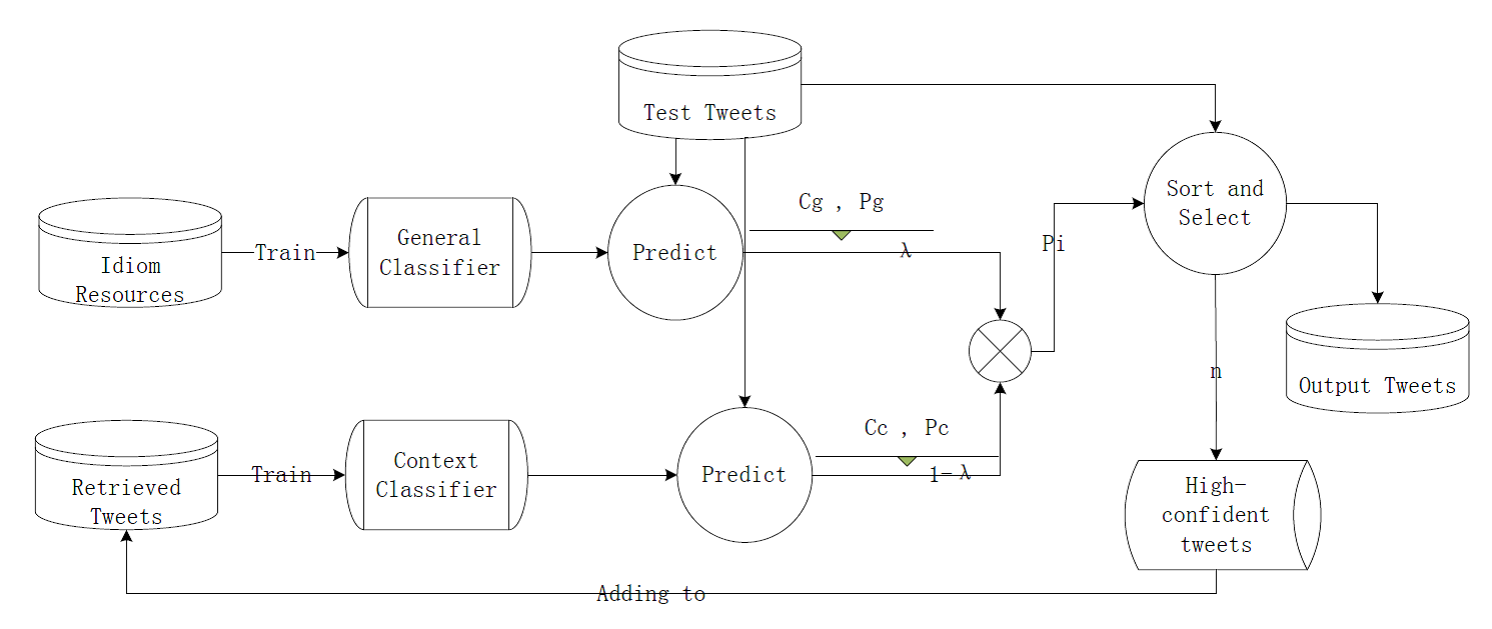
\includegraphics[width=550pt,height=350pt]{4-1.png}
\caption{自举式学习框架}
\label{fig4-1}
\end{figure*}
\end{landscape}
该框架中,我们要通过不断迭代训练学习到通用情感分类器$ P_{g} $和微博情感分类器$ P_{c} $,使得这两个分类器不但从单个视角达到分类性能的最优,也需要在对相同的测试数据上分类结果一致,组合性能能够提高。根据使用的分类器的不同,我们假设可以将分类器的输出用$  \lbrace p_{g},p_{c}\rbrace$来表示(例如SVM的距离输出或生成模型的概率输出)来表示分类结果的可信度。对于每一个待分类测试数据,首先使用两个情感分类器对其进行分类,预测其情感倾向性标签为$ c_{i}=\lbrace c_{g},c_{c}\rbrace $,并输出可信度$ p_{i}= \lbrace p_{g},p_{c}\rbrace$,然后将可信度按照公式~\ref{eq4-3}合成为一个:

\begin{equation}
\label{eq4-3}
p_{i}=\begin{cases}
& \lambda\ast p_{g} + \left( 1-\lambda \right) \ast p_{c} \qquad \mbox{if} \quad c_{g}=c_{c};\\
& 0 \qquad \textit{if} \quad c_{g} \neq c_{c};
\end{cases}.
\end{equation}
其中$ \lambda $是控制不同部分特征影响权重的系数,首先将其初始化为$ \lambda = 0.5 $,然后随着迭代的进行逐步增加$ \lambda $以使得组合起来的分类器逐步适应针对微博的情感分类。
根据两个分类器对每个测试数据预测情感标签 $ c_{i} \left( c_{i} \in \lbrace 1, -1\rbrace \right)$,将测试数据分为两组,并分别按照预测输出的的组合可信度的降序排列。在排序的两组数据中分别取其前$ n $ 条可信度最高的微博数据作为新的依赖于微博语境的微博情感分类器的训练数据加入到训练集中,以逐步提高该分类器对微博情感分类的适应性。这样的过程循环多次进行迭代,直至所有数据的情感分类组合可信度的变化因为小于某个指标而收敛。

总体来说,整个框架可以被视作是一个自举式(bootstrapping)共同训练(Co-training)\upcite{marchetti2012learning}机器学习算法过程,所不同的是该框架并没有使用标注好的训练数据,而是从现成的成语词典资源作为训练的起始点,是一个无监督的学习框架,因此节省了人工或自动标注微博数据的过程,对于数量庞大的微博数据来说,该框架更加实用。

\subsection{分类器算法}
\label{classifier}
对于两个分类器,我们采用跟Pang等~\upcite{Pang2002}文章中一样的三种机器学习算法:朴素贝页斯(Na\"\i ve Bayes)算法,最大熵(Maximum Entropy)算法以及支持向量机(Support Vector Machine)算法。这三种算法的有效性已经得到Pang等~\upcite{Pang2002}的验证,其中支持向量机取得的性能是最好的(准确率达到82.9\%)。

\subsubsection{Na\"\i ve Bayes分类器.}
\label{bayes}

Na\"\i ve Bayes在文本分类任务中是最常用的分类器。对与情感分类问题,为了确定一篇文档$ d_{i}$的情感倾向性类别$ c_{j} $,需要计算后验概率$ P \left(c_{j} \mid d_{i} \right)$。根据贝页斯法则和多项式分布,基于每一维特征概率的独立性假设,可以得到:

\begin{equation}
\label{e4}
P \left(c_{j} \mid d_{i} \right) = \frac{P \left( c_{j} \right)\prod_{k=1}^{| d_{i} |} P \left( w_{d_{i},k} \mid c_{j} \right)}{\sum_{r=1}^{|C|}P \left( c_{r} \right)\prod_{k=1}^{| d_{i} |} P \left( w_{d_{i},k} \mid c_{r} \right)} \enspace .
\end{equation}
通过计算每一情感类别的后验概率,概率最大的可以视为文档 $ d_{i} $的情感类别。

\subsubsection{最大熵分类器.}
\label{entropy}
最大熵(Maximum Entropy)分类器与Na\"\i ve Bayes分类器一样也是通过计算后眼概率来判断文档的情感类别,所不同的是最大熵分类器是计算条件概率:

\begin{equation}
\label{e5}
P \left( c_{j} \mid d_{i}, \overrightarrow{\theta} \right) = \frac{1}{Z}exp \left( \overrightarrow{\theta}, \overrightarrow{f} \left( d_{i},c_{j} \right) \right) \enspace .
\end{equation}
其中$ \overrightarrow{\theta} $表示特征向量,$ \overrightarrow{f} \left( d_{i}, c_{j} \right)$表示将训练实例$ \left( d_{i}, c_{j} \right) $映射到特征向量空间 的特征函数,$ Z $是归一化因子。
最大熵分类器用训练数据集$ D $的训练学习过程就是解一个最优化问题:

\begin{equation}
\label{e6}
\overrightarrow{\theta^{\ast}}=argmax_{\overrightarrow{\theta}}\prod_{i=1}^{|D|} P \left( c_{j} \mid d_{i}, \overrightarrow{\theta} \right) \enspace .
\end{equation} 

\subsubsection{支持向量机分类器.}
\label{svm}
支持向量机(Support Vector Machines)分类器是一种判别式的机器学习方法。支持向量机分类器的训练过程发现一个支持向量确定的决策平面将在训练数据能够分为两类,然后使用支持向量确定测试数据的类别。训练过程是接一个受限的最优化问题:

\begin{equation}
\label{e7}
\begin{aligned}
\overrightarrow{\alpha^{\ast}}=argmin \left( -\sum_{i=1}^{n}\alpha_{i} + \sum_{i=1}^{n} \sum_{j=1}^{n}\alpha_{i}\alpha{j} x_{i}x_{j}<\overrightarrow{x_{i}},\overrightarrow{x_{j}}> \right)\\
\mbox{Subject to:} \sum_{i=1}^{n}\alpha_{i}y_{i}=0 , 0\leqslant \alpha_{i} \leqslant 1
\end{aligned} \enspace .
\end{equation}
情感分类问题通常使用线性支持向量机分类器。

\section{实验}
\label{experiment}
为了验证所提出框架的性能,我们使用一部现成的在线成语词典和从腾讯微博\footnote{\url{http://t.qq.com/}}中抓取的数据进行了一系列的实验。

\subsection{实验描述}
\label{description}

\subsubsection{数据集}
我们从成语覆盖比较全的中国教育在线网\footnote{China Education Network:\url{http://chengyu.teachercn.com}}上抓取了在线的成语词典,经过整理的到了有8,160个条目的成语词典,其中褒义的(正面情感倾向)的成语有3,648条,贬义的(负面情感倾向)的成语有4,512条,我们使用这些数据训练通用情感分类器。
微博情感分类器的训练数据是通过腾讯微博公开API抓取的数据,从2013年四月15日开始到五月15日一个月的时间我们监控腾讯微博的实时数据流,查询抓取了至少含有一条成语的微博数据,形成120,346条微博数据的数据集。经过筛选过滤掉噪声和过短的数据,最后得到91,268条微博数据集用于训练微博情感分类器。
为了测试我们所提出的两种分类器组合形成的自举式分类器的性能,我们使用了中国计算机学会(CCF)举办的第一届自然语言处理与中文计算会议(Natural Language Processing and Chinese Computing)中的微博情感分析与语义关系抽取评测(the First Chinese tweet Sentiment Analysis and Semantic Relationship Extraction Evaluation)\footnote{\url{http://tcci.ccf.org.cn/conference/2012/pages/page04_eva.html}}的标注数据集作为测试数据。
 
\subsubsection{实验配置}
为了能够多角度测量分类器的性能,有各种评测指标,但是我们的实验不是为了比较这些评价指标的不同,因此我们选择了简单直观的准确率作为分类器性能的评价指标。
对于分类器,我们选择了自然语言处理的工具NLTK(Natural Language ToolKits)\upcite{Loper2002}中的Na\"\i ve Bayes分类器和最大熵分类器,以及常用的Libsvm\upcite{Chang2011}工具包的支持向量机分类器。
分类中所有的参数设置都经过交叉验证进行了优化。

\subsubsection{评价基准}
为了客观评价我们的方法的性能,我们设置了三个评价基准用于对比评价。一个是50\%的基准,因为我们所用的测试数据集是平衡数据集,所以即便是随机判断的分类器的准确率可以达到这样的准确率;第二个是用一个基于情感词典的情感分类器的准确率作为基准,我们使用的是前面两章构建的SentiHowNet情感词典,通过计算每条微博中的包含的情感词语情感值叠加来计算综合情感值,然后判断微博的情感倾向性;第三个基准是有监督的机器学习方法构建的情感分类器,我们按照Pang等~\upcite{Pang2002}文章中的方法使用测试数据通过5倍交叉验证方式训练了朴素贝页斯(Na\"\i ve Bayes)、最大熵(Maximum Entropy)以及支持向量机(Support Vector Machine)分类器,把三种分类器的在测试数据集上的准确性作为基准。

\subsubsection{数据预处理}
中文文本信息不像英文那样靠空格自然形成了词语结构,因此需要对中文进行分词预处理才能进行词袋特征的抽取。我们使用常用的中科院ICTCLAS\footnote{\url{http://ictclas.nlpir.org/}}分词软件上述所有数据进行分词处理,并进行了停用词过滤。

\subsection{实验结果}
\label{result}

为了确定公式~\ref{eq4-3}中的$ \lambda $值,我们从0到1对$ \lambda $值进行了遍历实验,每一遍历步$ \lambda $值增加0.1,实验结果如图~\ref{fig4-2}所示。

\begin{figure}[htp]
\centering
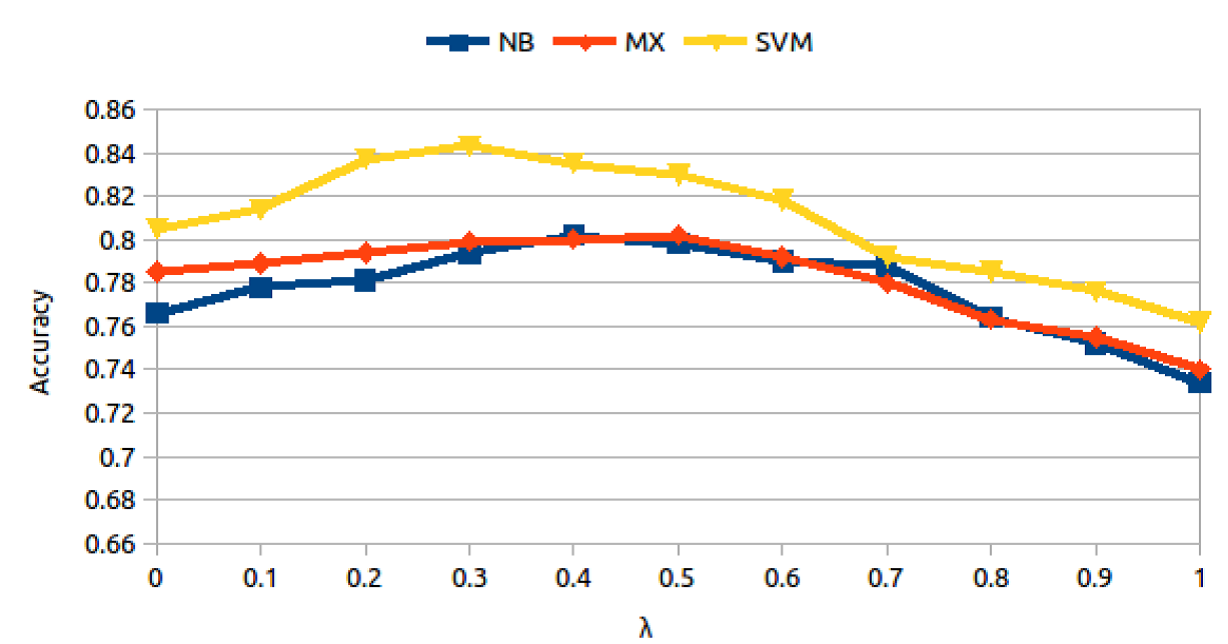
\includegraphics[height=230pt]{4-2.png}
\caption{$ \lambda $值的确定。}
\label{fig4-2}
%\description{NB代表 Na\"\i ve Bayes分类器,MX代表最大熵分类器,SVM代表支持向量机分类器。}
\end{figure}
从图中可以确定对于三种分类器所确定的$ \lambda $值:对于Na\"\i ve Bayes分类器,$ \lambda=0.4 $;对于最大熵分类器,$ \lambda=0.5 $;对于支持向量机分类器,$ \lambda=0.3 $。

确定了$ \lambda$后,经过自举式的学习训练,并在测试集上评价,最后的结果如表~\ref{tab4-1}所示。

\begin{table}[htp]
\caption{结果对比表}
\label{tab4-1}
\centering
\begin{tabular}{|l||l|l|l|}
\hline
\bfseries Classifier &  \bfseries NB    &   \bfseries MX    &   \bfseries SVM    \\
\hline

\bfseries Lexicon Classifier & 0.725 & 0.725 & 0.725 \\
\hline
\bfseries Supervised Classifier & 0.785 & \textbf{0.806} & 0.826 \\
\hline
\bfseries General Classifier & 0.734 &  0.740 & 0.762 \\
\hline
\bfseries Context Classifier & 0.766 & 0.785 & 0.805 \\
\hline
\bfseries Combined Classifier & \textbf{0.802} & 0.802 & \textbf{0.843} \\
\hline
\end{tabular}
\end{table}
从表中可以看出,首先无论是通用情感分类器还是微博情感分类器,性能上都超过了随机基准的50\%准确率,这证明了无论是从那种视角进行分类,两种分类器都是有效的,胜过随机猜测。因此在没有任何标注数据来训练有监督或半监督分类器的情况下,我们的特征分割假设可以作为情感分类的一种有效的方法。

其次,通用情感分类器的准确率比基于情感词典的分类器要稍微好些,这是因为尽管通用情感分类器和基于词典的分类器都使用领域独立的词语来对情感知识进行建模,但是通用情感分类器是经过成语等知识资源所抽取的特征空间进行训练的,而情感词典中的词语都是独立使用并且还是具有一定的歧义;而对于微博情感分类器,准确率都比基于词典的分类器和通用情感分类器要好,因为它是使用微博依赖部分的特征训练得到的,更能使用微博语言环境,测试数据中出现的微博的“火星语言”越多越能体现出微博情感分类器的性能优越性。

最后,使用自举式学习框架的组合分类器显示出了最好的性能,因为它结合了通用分类器和微博分类器的综合性能,其准确率也超过了准确率比较高的有监督的分类器,这说明我们提出的方法既能很好的利用通用情感表达知识把握微博的总体情感倾向,也能照顾到微博特有的情感表达方式,准确掌握微博中细致的情感倾向。

\section{小结}
\label{conclusion}
本章中我们针对情感分类的领域依赖性问题提出了无监督的自举式学习框架,并在微博中进行了验证。通过将情感分类问题的特征空间进行多视角分割,将整个特征向量特征空间分为领域独立的通用特征部分和领域依赖的微博特征空间,因此可以在两个特征空间分别训练得到通用情感分类器和微博情感分类器。然后我们使用了自举式的机器学习框架将两种分类器组合起来,达到更好的分类效果。实验证明我们所提出的方法性能上超过了现有的主要一些情感分类方法。